\chapter{Compact Muon Solenoid}

\section{Introduction}
About 100 meters below the town of Cessy, France at Point 5 is the Compact Muon Solenoid (CMS).  The CMS is a general purpose detector weighing 14,000 tonnes with a length of 28.7 meters and a 15.0-meter diameter that was designed to accurately measure the energy and momentum of particles produced in the proton-proton or heavy-ion collisions at the LHC \cite{Collaboration_2008}.  A perspective view of of the detector is shown in Figure \ref{fig:cmsschematic}.  In order to get a full picture of what is being produced by the collisions the CMS detector must be able identify the resulting particles as well as accurately measure their energy and momentum.  For this reason the detector was designed to be a collection of specialized sub-detectors, each of which contributes data used in the reconstruction of a collision.  
\begin{figure}[h]
	\centering
	\includegraphics[width=0.7\linewidth]{Figures/cms_schematic}
	\caption{Schematic of CMS detector \cite{Sakuma_2014}}
	\label{fig:cmsschematic}
\end{figure}

At the heart of the CMS detector is a 3.8-Tesla magnetic field produced by a superconducting solenoid.  Inside the 6-meter diameter solenoid are three layers of sub-detectors.  These make up the inner detector and are, in order from innermost to outermost, the silicon tracker, the electromagnetic calorimeter (ECAL), and the hadronic calorimeter (HCAL).  Outside the solenoid is the muon system.  A transverse slice of the detector (Figure \ref{fig:cmsslicewhitecolourfrench291016}) shows the sub-detectors and how different types of particles interact with with them.  Table \ref{table:subdetsignals} shows a summary of which sub-detectors are expected to produce signals for different types of particles.

\begin{figure}[h]
	\centering
	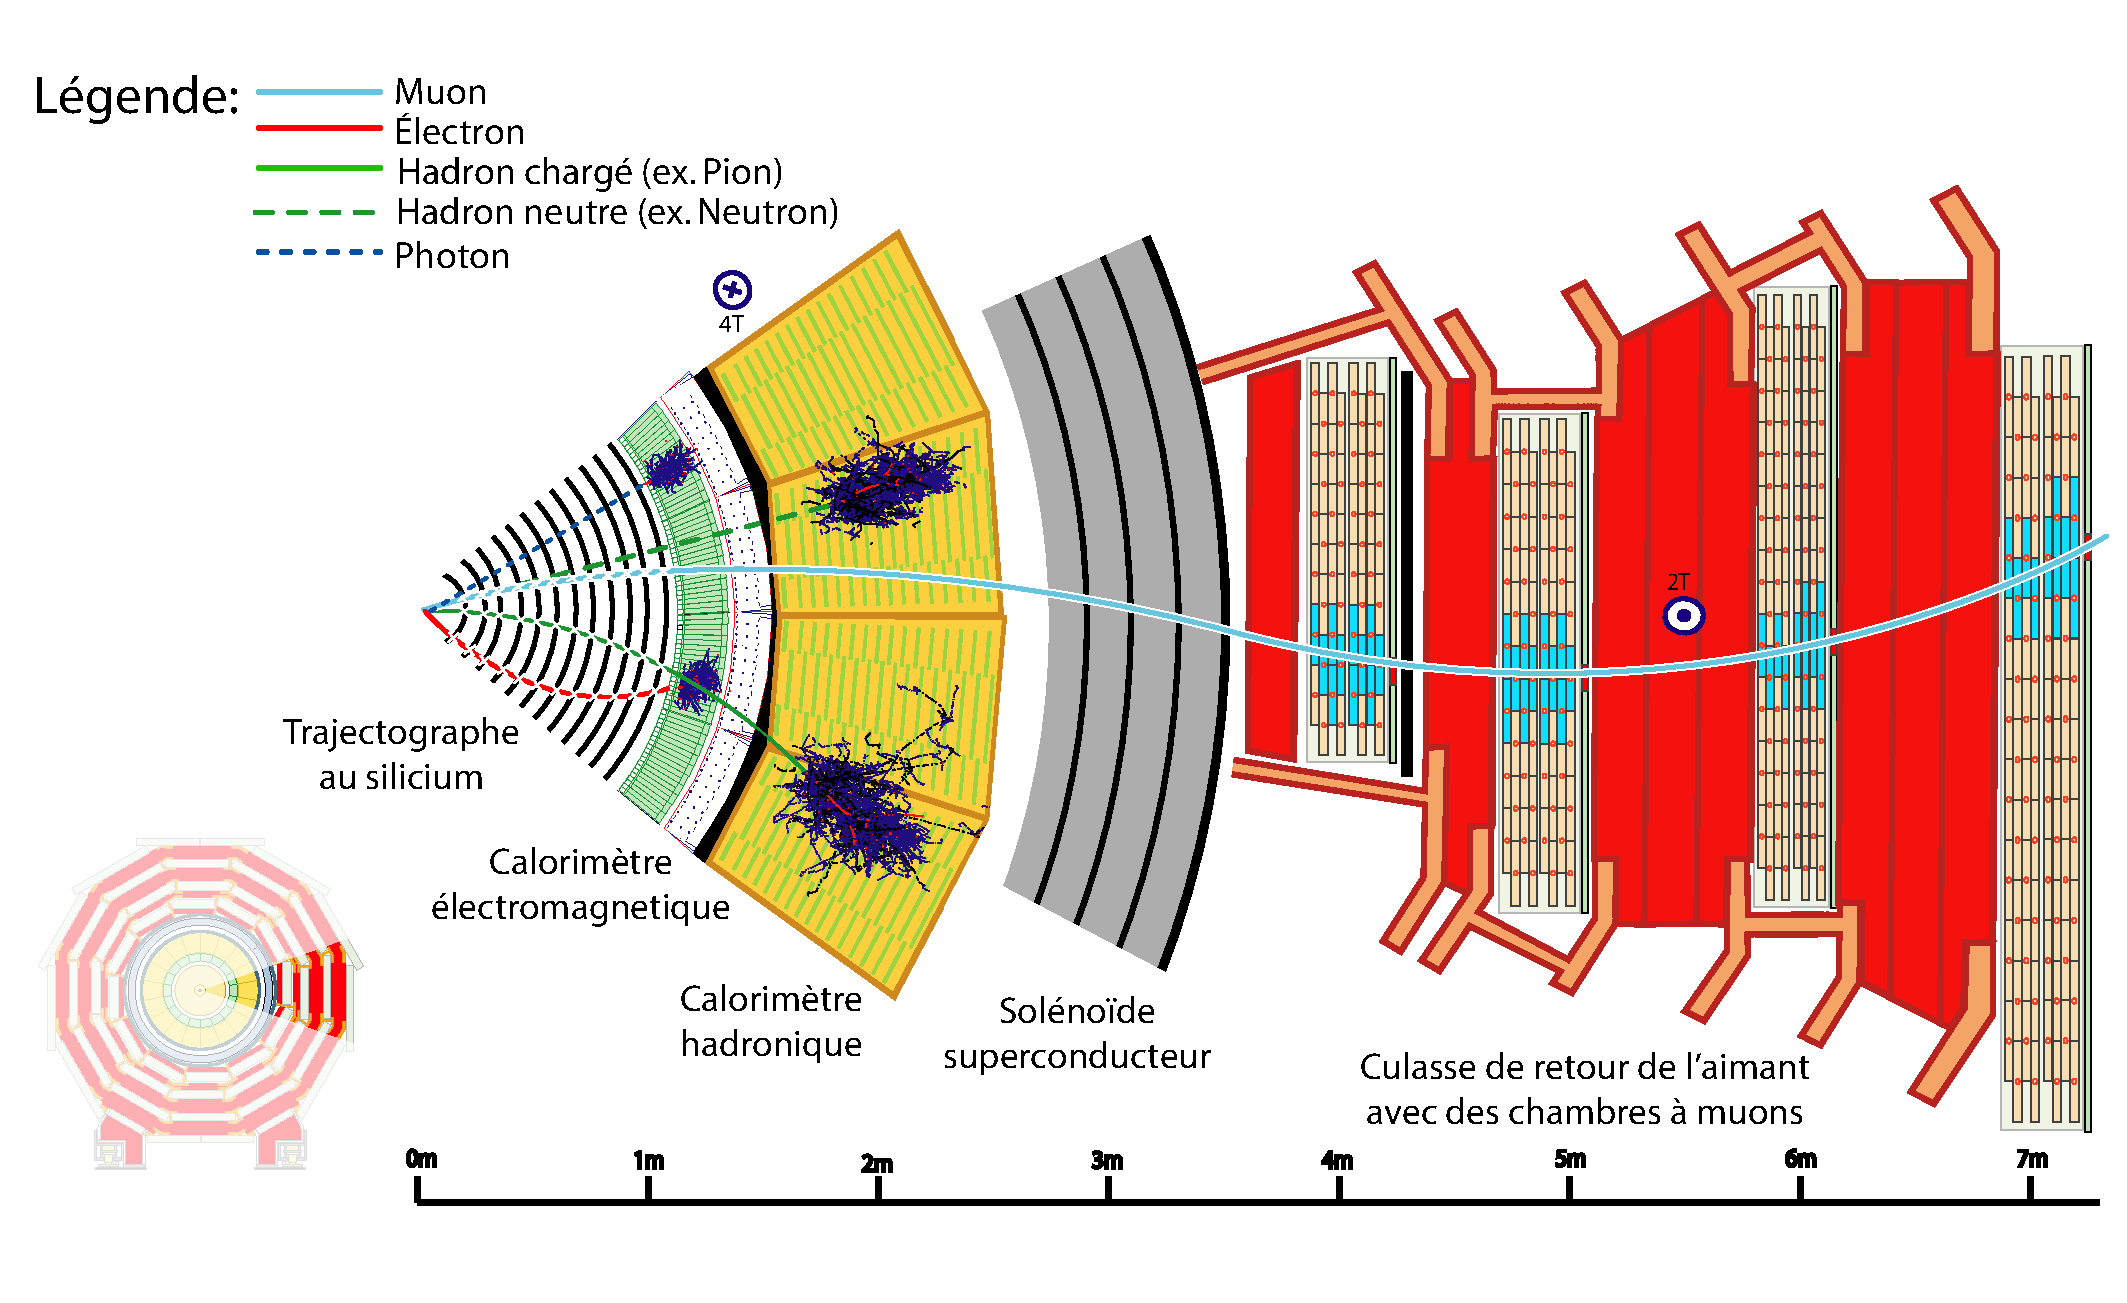
\includegraphics[width=0.7\linewidth]{Figures/CMS_slice_white_colour_french_291016}
	\caption{Transverse slice of the CMS detector\cite{Barney:2628641}.}
	\label{fig:cmsslicewhitecolourfrench291016}
\end{figure}



\begin{table}[h]
	\centering
\begin{tabular}{|c|c|c|c|c|}
	\hline 
	Particle & Tracker & ECAL & HCAL & Muon \\ 
	\hline 
	Photons & No & Yes & No & No \\ 
	\hline 
	Electrons & Yes & Yes & No & No \\ 
	\hline 
	Hadrons (charged) & Yes & No & Yes & No \\ 
	\hline 
	Hadrons (neutral) & No & No & Yes & No \\ 
	\hline 
	Muons & Yes & No & No & Yes \\ 
	\hline 
	Invisible ($\nu$, SUSY, etc) & No & No & No & No \\ 
	\hline 
\end{tabular} 
\caption{Summary of signals expected for each particle type in each sub-detector}
\label{table:subdetsignals}
\end{table}


\section{Coordinate System}
The origin of the coordinate system used by CMS is centered at the nominal collision point in the center of the detector.  A right-handed Cartesian system is used with the x-axis pointing radially inward toward the center of the LHC ring, y-axis pointing vertically upward, and the z-axis pointing tangent to the LHC ring in the counterclockwise direction as viewed from above.  CMS also uses an approximately Lorentz invariant spherical coordinate system spanned by three basis vectors.  They are the transverse momentum $p_{T}$, pseudorapidity $\eta$, and azimuthal angle $\phi$.  The transverse momentum and azimuthal angle translate to the Cartesian system in the following ways using the x and y-components of the linear momentum:
\begin{equation}
p_{T} = \sqrt{(p_{x})^{2} + (p_{y})^{2}}
\end{equation}
\begin{equation}
\phi = tan^{-1}\frac{p_{y}}{p_{x}}
\end{equation}
while the pseudorapidity can be translated using the polar angle $\theta$ relative the positive z-axis as
\begin{equation}
\eta = -ln[tan\frac{\theta}{2}].
\end{equation}


\section{Tracker}
The innermost sub-detector in CMS is the silicon tracker.  The tracker is used to reconstruct tracks and vertices of charged particles.  In order to give precise reconstruction of charged particle trajectories needs to be position as close as possible to the IP and have high granularity.  The close proximity to the IP requires the materials to be tolerant to the high levels of radiation in that region.  Being the innermost sub-detector it must also minimally disturb particles as they pass through it into the other sub-detectors.  These criteria led to the design of the tracker using silicon semiconductors.

The silicon tracker is made up of two subsystems, an inner pixel detector and an outer strip tracker which are oriented in a cylindrical shape with an overall diameter of 2.4 m and length of 5.6 m centered on the interaction point.  Both subsystems consist of barrel and endcap regions which can be seen in Figure \ref{fig:trackerlayoutv2}.  

\begin{figure}[h]
	\centering
	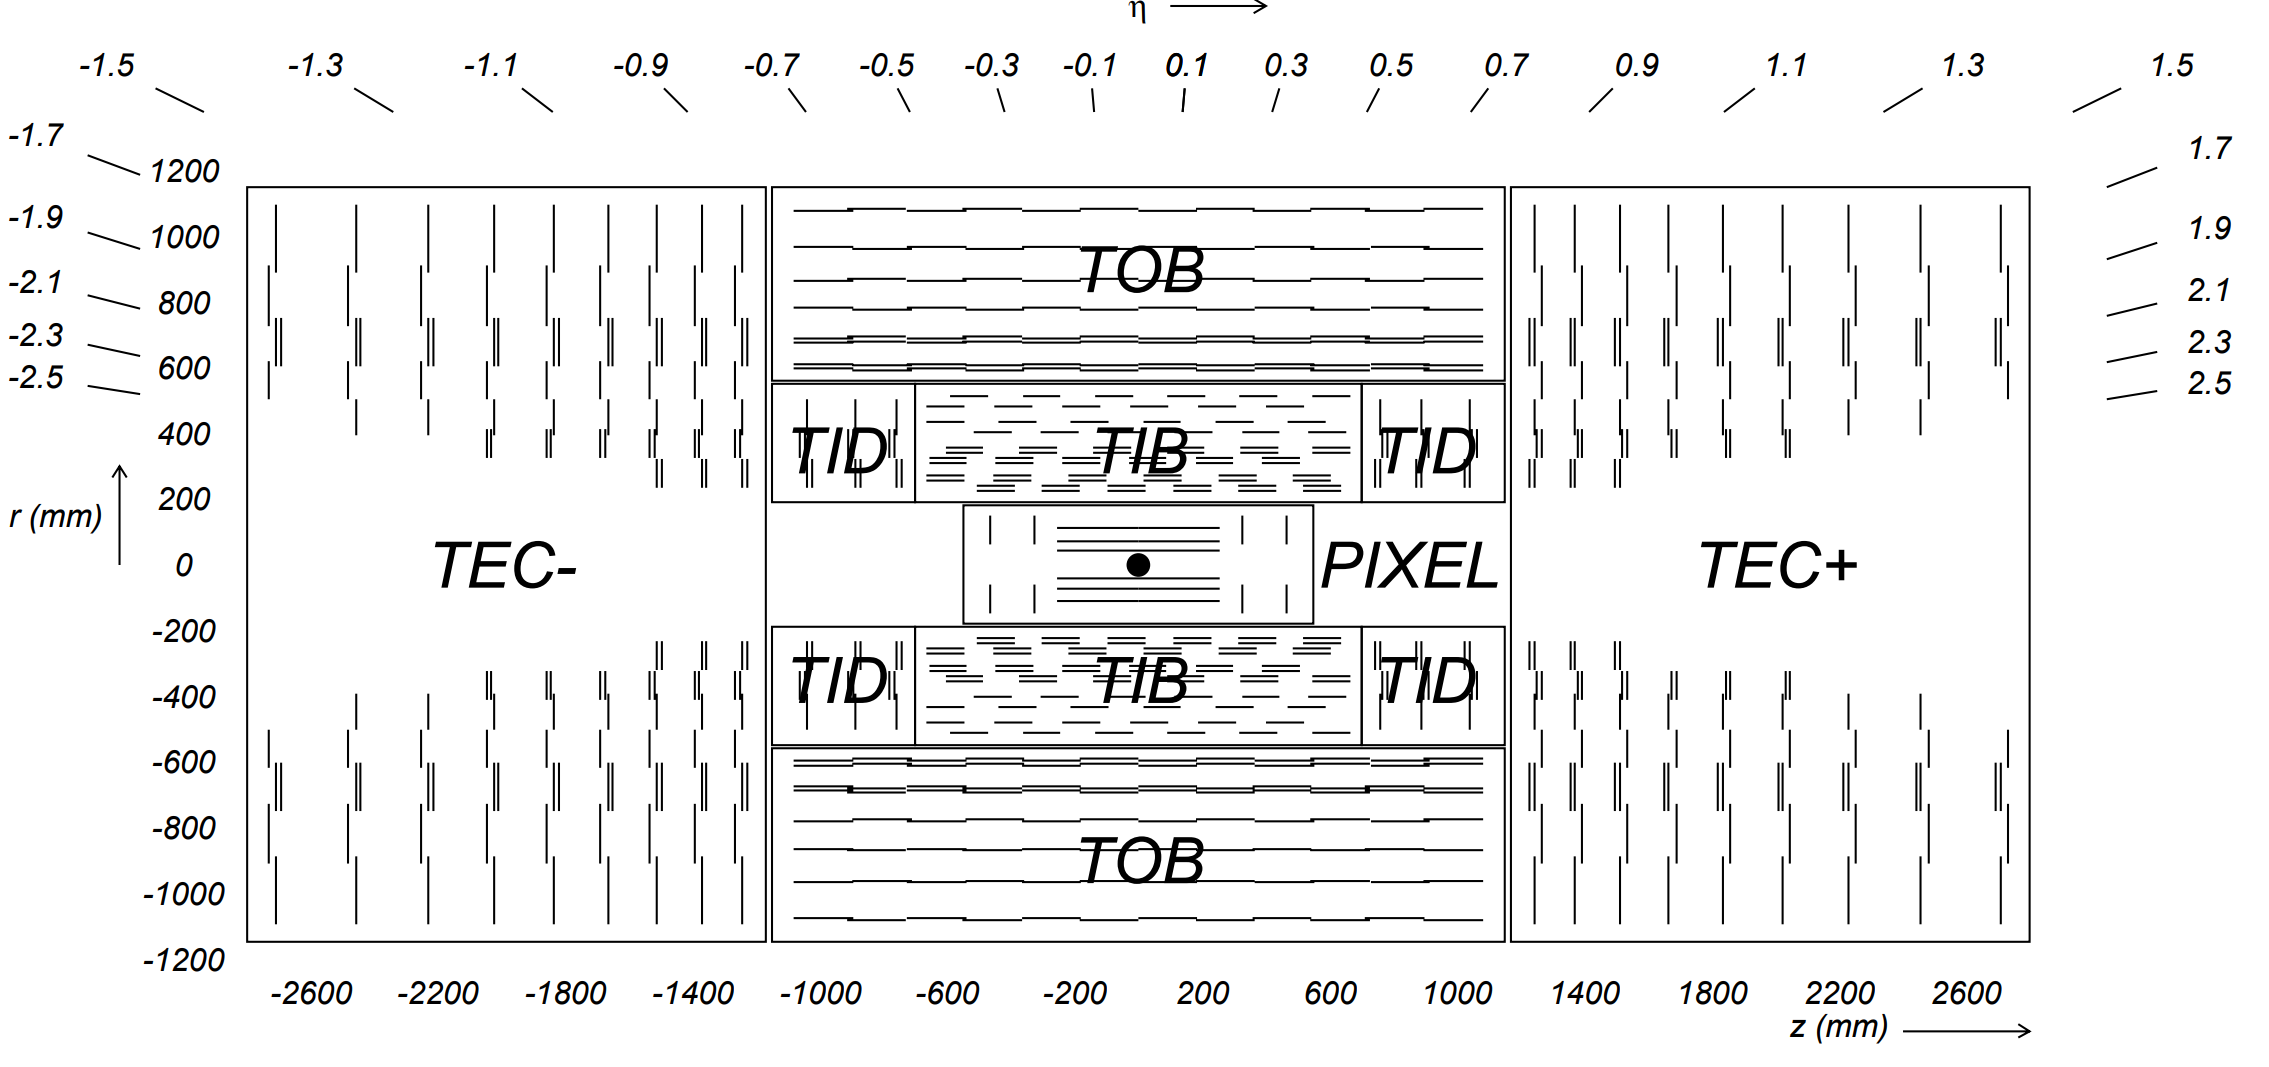
\includegraphics[width=0.7\linewidth]{Figures/TrackerLayout_v2}
	\caption{Cross section (side) of CMS tracker prior to the Phase 1 upgrade during the year-end technical stop of 2016/2017. Each line represents a detector module while double lines indicate back-to-back strip modules. Surrounding the pixel tracker (PIXEL) is the strip detector, which is divided into the Tracker Inner Barrel (TIB), Tracker Outer Barrel (TOB), Tracker Inner Disk (TID), and Tracker Endcap (TEC). Reprinted from Reference \cite{Chatrchyan:1704291}.}
	\label{fig:trackerlayoutv2}
\end{figure}

\subsection{Pixel Detector}
The pixel detector is the innermost subsystem in the silicon tracker.  Pixels were used here rather than strips because at this distance from IP one expects there to be high occupancy of the tracker.  The original pixel detector was designed for operation at the nominal instantaneous luminosity of 10$^{34}$ cm$^{-2}$s$^{-1}$ with 25 ns between proton bunch crossings, resulting in on average about 25 proton-proton interactions occurring per bunch crossing or pileup.  During the LHC technical shutdown of 2016/17, the pixel detector underwent the scheduled Phase 1 upgrade which would allow operation at higher levels of instantaneous luminosity and pileup.  Figure \ref{fig:trackersideview} shows a cross sectional view in the \textit{r-z} plane.  Prior to 2017 there were three barrel layers and two endcap layers on each side which provide three very precise space points for each charged particle.  The upgrade decreased the radius of the innermost barrel layer from 4.4 cm to 3.0 cm and added a fourth barrel layer as well as adding third endcap layer to each side.  Each of the endcap layers consisted of two half-disks populated with pixel modules whereas the upgraded endcap layers were split into inner and outer rings. \cite{Dominguez:1481838}

\begin{figure}[h]
	\centering
	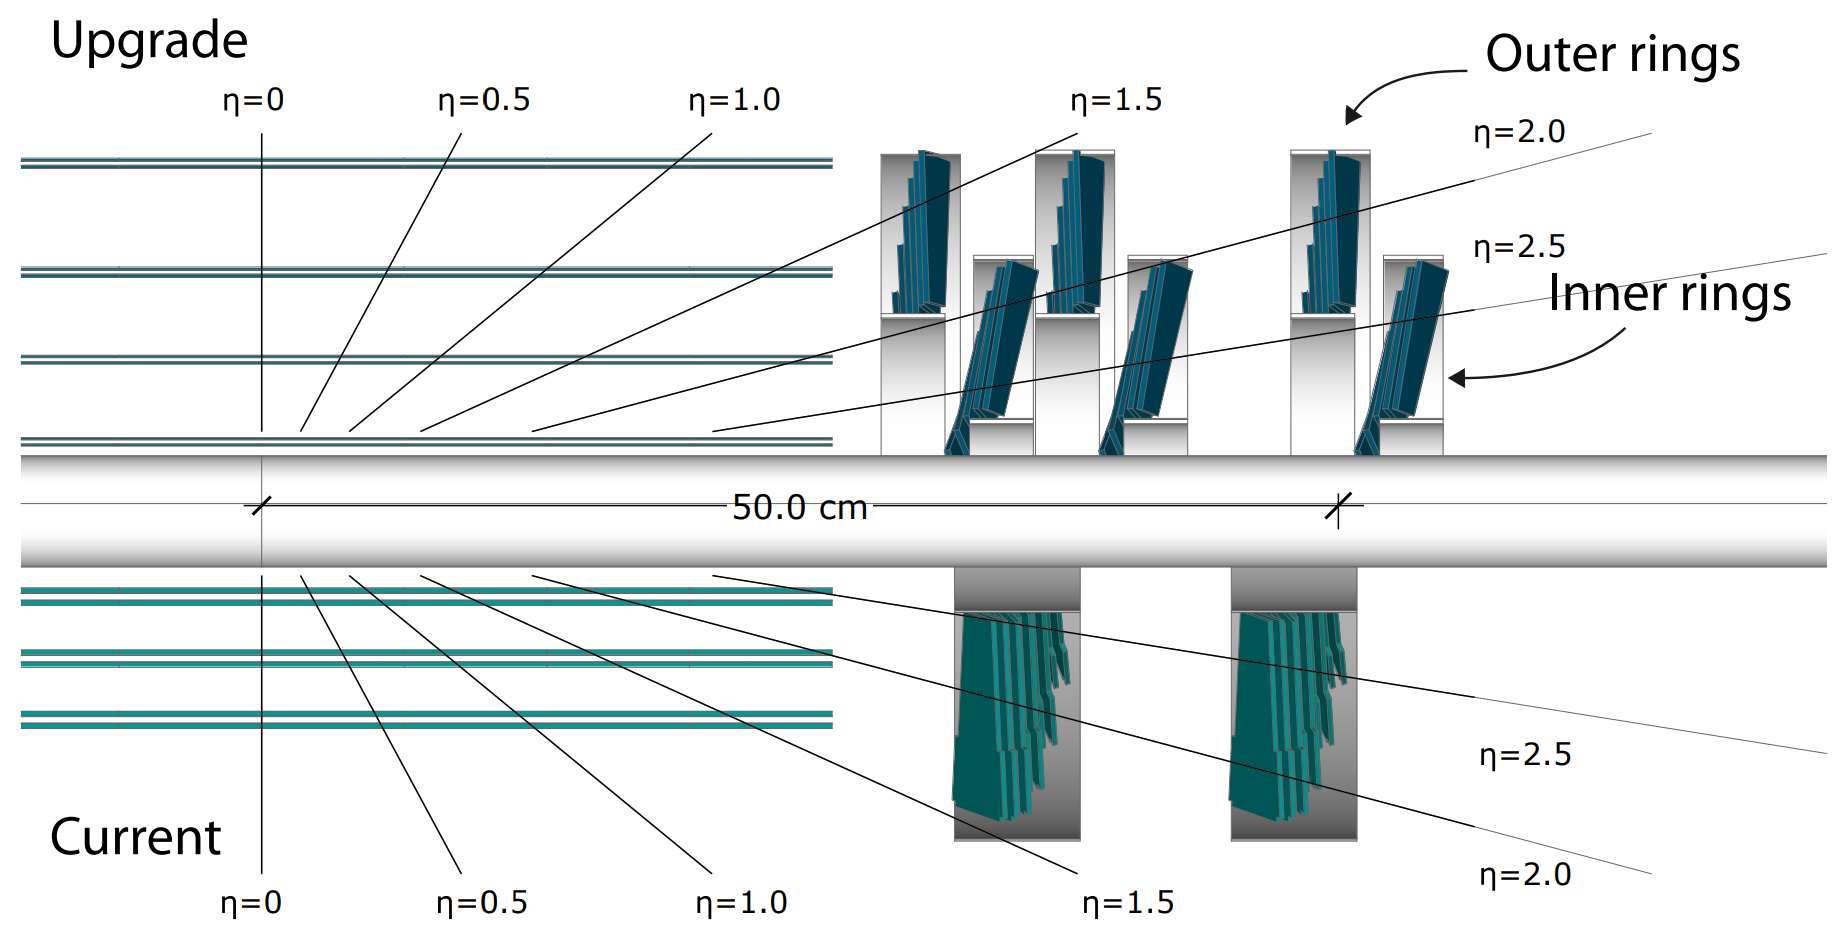
\includegraphics[width=0.7\linewidth]{Figures/Tracker_sideview}
	\caption{Cross section (side) of pixel detector. The lower half , labeled "Current", shows the design prior to 2017 while the upper half, labeled "Upgrade", shows the design after the upgrade. Reprinted from Resource \cite{Dominguez:1481838}}
	\label{fig:trackersideview}
\end{figure}





\section{Electromagnetic Calorimeter}

\section{Hadronic Calorimeter}

\section{Muon System}

